\documentclass[12pt,a4paper]{article}

%% ============================================================
%%  PACKAGES
%% ============================================================
\usepackage[a4paper, margin=2.5cm]{geometry}
\usepackage{amsmath, amssymb, amsthm}
\usepackage{fancyhdr}
\usepackage[dvipsnames,svgnames,x11names]{xcolor}
\usepackage{tikz}
\usetikzlibrary{shapes, arrows.meta, positioning, backgrounds,
                patterns, decorations.pathreplacing, calc, quotes}
\usepackage{float}
\usepackage{hyperref}
\usepackage{mathtools}
\usepackage{enumitem}
\usepackage{microtype}
\usepackage{titlesec}
\usepackage{booktabs}

%% ============================================================
%%  THEOREM ENVIRONMENTS
%% ============================================================
\theoremstyle{definition}
\newtheorem{definition}{Definition}[section]
\newtheorem{example}{Example}[section]

\theoremstyle{plain}
\newtheorem{theorem}{Theorem}[section]
\newtheorem{lemma}{Lemma}[section]
\newtheorem{corollary}{Corollary}[section]
\newtheorem{proposition}{Proposition}[section]

\theoremstyle{remark}
\newtheorem{remark}{Remark}[section]

%% ============================================================
%%  PAGE STYLE
%% ============================================================
\pagestyle{fancy}
\fancyhf{}
\fancyhead[L]{\small\leftmark}
\fancyhead[R]{\small\thepage}
\fancyfoot[C]{\small Lecture Notes: Planar Graphs and Graph Colorings}
\renewcommand{\headrulewidth}{0.4pt}
\renewcommand{\footrulewidth}{0.4pt}

%% ============================================================
%%  TITLE / SECTION FORMATTING
%% ============================================================
\titleformat{\section}{\large\bfseries}{§\,\thesection.}{0.5em}{}[\titlerule]
\titleformat{\subsection}{\normalsize\bfseries}{\thesubsection.}{0.5em}{}

%% ============================================================
%%  HYPERREF SETUP
%% ============================================================
\hypersetup{
  colorlinks=true,
  linkcolor=black,
  citecolor=ForestGreen,
  urlcolor=Crimson,
  pdftitle={Lecture Notes: Planar Graphs and Graph Colorings},
  pdfauthor={Prof. Name Surname}
}

%% ============================================================
%%  TIKZ STYLES
%% ============================================================
\tikzset{
  vertex/.style={circle, draw=black, fill=black,
                 inner sep=0pt, minimum size=6pt},
  vertexW/.style={circle, draw=black, fill=white,
                  inner sep=1pt, minimum size=18pt, font=\small},
  redV/.style={circle, draw=black, fill=Crimson,
               inner sep=1pt, minimum size=18pt, font=\small\color{white}},
  blueV/.style={circle, draw=black, fill=RoyalBlue,
                inner sep=1pt, minimum size=18pt, font=\small\color{white}},
  greenV/.style={circle, draw=black, fill=ForestGreen,
                 inner sep=1pt, minimum size=18pt, font=\small\color{white}},
  yellowV/.style={circle, draw=black, fill=Goldenrod,
                  inner sep=1pt, minimum size=18pt, font=\small},
  orangeV/.style={circle, draw=black, fill=DarkOrange,
                  inner sep=1pt, minimum size=18pt, font=\small\color{white}},
  purpleV/.style={circle, draw=black, fill=DarkViolet,
                  inner sep=1pt, minimum size=18pt, font=\small\color{white}},
  edge1/.style={draw=Crimson, line width=1.4pt},
  edge2/.style={draw=RoyalBlue, line width=1.4pt},
  edge3/.style={draw=ForestGreen, line width=1.4pt},
}

%% ============================================================
%%  DOCUMENT
%% ============================================================
\begin{document}

%% ---- TITLE PAGE -------------------------------------------
\begin{titlepage}
    \centering
    \vspace*{4cm}
    
    {\Huge\bfseries Lecture Notes:\\ Planar Graphs
and Graph Colorings\par}
    \vspace{1cm}
    {\Large Discrete Mathematics\par}
    \vspace{2cm}
    {\large \textbf{Author:} Bakdaulet Sotsial\par}
    \vspace{1cm}
    
    \vfill
    {\small Astana IT University \par}
    \vspace*{2cm}
\end{titlepage}

\thispagestyle{empty}
\tableofcontents
\newpage

%% ===========================================================
%%  SECTION 1: PLANAR GRAPHS
%% ===========================================================
\section{Planar Graphs — Definitions and Basic Concepts}
\label{sec:planar-def}

We begin by establishing the foundational vocabulary of planarity.  Throughout
these notes, a \emph{graph} $G=(V,E)$ is a finite, simple, undirected graph
unless stated otherwise.

\begin{definition}[Planar graph]\label{def:planar}
  A graph $G$ is said to be \textbf{planar} if it can be drawn in the Euclidean
  plane $\mathbb{R}^{2}$ in such a way that no two edges cross one another
  (except possibly at shared endpoints).
\end{definition}

\begin{definition}[Plane graph / planar embedding]\label{def:plane}
  A \textbf{plane graph} is a particular drawing (embedding) of a planar graph
  in the plane in which no two edges intersect except at their common endpoints.
  Such a drawing is called a \textbf{planar embedding} of $G$.
\end{definition}

\begin{remark}\label{rem:plane-vs-planar}
  The distinction between \emph{planar} and \emph{plane} is important: ``planar''
  is an intrinsic property of the abstract graph, while ``plane graph'' refers
  to a concrete drawing.  A single planar graph may admit many non-equivalent
  plane embeddings.
\end{remark}

\begin{definition}[Faces of a plane graph]\label{def:faces}
  Let $G$ be a plane graph.  The complement $\mathbb{R}^{2}\setminus G$ (the
  plane minus the drawing of $G$) is an open set whose connected components are
  called the \textbf{faces} (or \textbf{regions}) of $G$.
\end{definition}

By the Jordan Curve Theorem, every simple closed curve in $\mathbb{R}^2$ divides
the plane into exactly two components.  Consequently:

\begin{itemize}
  \item Exactly one face is \textbf{unbounded} (extends to infinity); it is
        called the \textbf{outer face} or \textbf{exterior face}.
  \item All remaining faces are \textbf{bounded} (finite regions enclosed by
        edges).
\end{itemize}

\begin{definition}[Boundary walk and face degree]\label{def:face-degree}
  The \textbf{boundary walk} of a face $f$ is the closed walk that traces the
  edges incident to $f$.  The \textbf{degree} of $f$, denoted $\deg(f)$, is
  the number of edges in this boundary walk (counting each edge at most twice
  if it borders $f$ on both sides).
\end{definition}

\begin{example}[Planar embedding of $K_4$]\label{ex:K4}
  The complete graph $K_4$ on four vertices is planar.  Figure~\ref{fig:K4}
  shows a planar embedding.  This embedding has $v=4$ vertices, $e=6$ edges,
  and $f=4$ faces (three bounded triangular faces $f_1,f_2,f_3$ and one
  unbounded outer face $f_4$).  The reader may verify: $4-6+4=2$.
\end{example}

\begin{figure}[htbp]
  \centering
  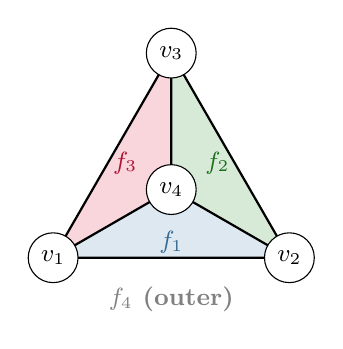
\begin{tikzpicture}[scale=1.5]
    %% vertices
    \coordinate (v1) at (0,0);
    \coordinate (v2) at (2,0);
    \coordinate (v3) at (1,1.732);
    \coordinate (v4) at (1,0.577);

    %% shaded faces
    \begin{scope}[on background layer]
      %% f1 – bottom-left triangle v1 v2 v4
      \fill[SteelBlue, fill opacity=0.18]
            (v1) -- (v2) -- (v4) -- cycle;
      %% f2 – bottom-right triangle v2 v3 v4
      \fill[ForestGreen, fill opacity=0.18]
            (v2) -- (v3) -- (v4) -- cycle;
      %% f3 – top-left triangle v1 v3 v4
      \fill[Crimson, fill opacity=0.18]
            (v1) -- (v3) -- (v4) -- cycle;
    \end{scope}

    %% edges
    \draw[thick] (v1)--(v2) (v1)--(v3) (v1)--(v4)
                 (v2)--(v3) (v2)--(v4) (v3)--(v4);

    %% vertex labels
    \node[vertexW] at (v1) {$v_1$};
    \node[vertexW] at (v2) {$v_2$};
    \node[vertexW] at (v3) {$v_3$};
    \node[vertexW] at (v4) {$v_4$};

    %% face labels
    \node[font=\small\bfseries, color=SteelBlue!80!black]
          at ($(v1)!0.5!(v2)!0.22!(v4)$) {$f_1$};
    \node[font=\small\bfseries, color=ForestGreen!80!black]
          at ($(v2)!0.5!(v3)!0.22!(v4)$) {$f_2$};
    \node[font=\small\bfseries, color=Crimson!80!black]
          at ($(v1)!0.5!(v3)!0.22!(v4)$) {$f_3$};
    \node[font=\small\bfseries, color=gray]
          at (1,-0.35) {$f_4$ (outer)};
  \end{tikzpicture}
  \caption{A planar embedding of $K_4$.  The three shaded regions are the bounded
           faces $f_1, f_2, f_3$; the exterior region is the outer face $f_4$.}
  \label{fig:K4}
\end{figure}

%% ===========================================================
%%  SECTION 2: EULER'S FORMULA
%% ===========================================================
\section{Euler's Formula and Consequences}
\label{sec:euler}

\subsection{Euler's Formula}

\begin{theorem}[Euler's Formula, 1758]\label{thm:euler}
  Let $G$ be a connected plane graph with $v$ vertices, $e$ edges, and $f$
  faces.  Then
  \[
    v - e + f = 2.
  \]
\end{theorem}

\begin{proof}
  We proceed by induction on the number of edges $e$.

  \medskip\noindent
  \textbf{Base case ($e = v-1$).}  Since $G$ is connected and has $e=v-1$
  edges, $G$ is a spanning tree.  A tree has no cycles, so its plane embedding
  has exactly one face (the outer face), i.e.\ $f=1$.  Then
  \[
    v - e + f = v - (v-1) + 1 = 2. \qquad\checkmark
  \]

  \medskip\noindent
  \textbf{Inductive step.}  Suppose the formula holds for all connected plane
  graphs with fewer than $e$ edges, where $e \geq v$.  Let $G$ be a connected
  plane graph with $v$ vertices and $e$ edges.  Since $e \geq v > v-1$, $G$
  contains at least one cycle, so there exists an edge $\ell \in E(G)$ that lies
  on a cycle.

  Remove $\ell$ to obtain the plane graph $G' = G - \ell$.  Since $\ell$ lies on
  a cycle, its removal does not disconnect $G$, so $G'$ is still connected.
  Moreover, $\ell$ is incident to exactly two distinct faces in $G$; removing it
  merges those two faces into one.  Therefore $G'$ has
  \[
    v' = v, \quad e' = e-1, \quad f' = f-1.
  \]
  By the inductive hypothesis applied to $G'$:
  \[
    v' - e' + f' = 2
    \;\Longrightarrow\;
    v - (e-1) + (f-1) = 2
    \;\Longrightarrow\;
    v - e + f = 2.
  \]
  This completes the induction.
\end{proof}

\subsection{Corollaries of Euler's Formula}

We now derive several important consequences.  Throughout, $G$ denotes a
connected simple planar graph unless stated otherwise.

\begin{corollary}\label{cor:3v6}
  If $G$ is a connected simple planar graph with $v \geq 3$ vertices and $e$
  edges, then
  \[
    e \leq 3v - 6.
  \]
\end{corollary}

\begin{proof}
  Fix any planar embedding of $G$.  Since $G$ is simple and $v \geq 3$, every
  face has degree at least $3$ (each face is bounded by at least a triangle).
  Summing face degrees:
  \begin{align}
    \sum_{i=1}^{f} \deg(f_i) &\geq 3f. \label{eq:facesum1}
  \end{align}
  On the other hand, each edge borders exactly two faces (or the same face
  twice), so
  \begin{align}
    \sum_{i=1}^{f} \deg(f_i) &= 2e. \label{eq:facesum2}
  \end{align}
  Combining \eqref{eq:facesum1} and \eqref{eq:facesum2}: $2e \geq 3f$, i.e.\
  $f \leq \tfrac{2e}{3}$.  Substituting into Euler's formula
  $v - e + f = 2$:
  \[
    2 = v - e + f \leq v - e + \frac{2e}{3} = v - \frac{e}{3},
  \]
  whence $e \leq 3v - 6$.
\end{proof}

\begin{corollary}\label{cor:deg5}
  Every simple planar graph $G$ contains a vertex of degree at most $5$.
\end{corollary}

\begin{proof}
  Suppose for contradiction that every vertex has degree at least $6$.  Then the
  sum of degrees satisfies $\sum_{v} \deg(v) \geq 6v$.  By the handshaking lemma,
  $2e \geq 6v$, so $e \geq 3v$.  But by Corollary~\ref{cor:3v6}, $e \leq 3v-6$,
  giving $3v \leq 3v - 6$, a contradiction.
\end{proof}

\begin{corollary}\label{cor:K5}
  The complete graph $K_5$ is non-planar.
\end{corollary}

\begin{proof}
  $K_5$ has $v=5$ and $e=10$.  By Corollary~\ref{cor:3v6}, any simple planar
  graph on $5$ vertices satisfies $e \leq 3(5)-6 = 9 < 10$.  Hence $K_5$ is
  not planar.
\end{proof}

\begin{corollary}\label{cor:2v4}
  If $G$ is a connected simple planar graph with $v \geq 3$ vertices, $e$ edges,
  and girth at least $4$ (i.e.\ $G$ contains no triangle), then
  \[
    e \leq 2v - 4.
  \]
\end{corollary}

\begin{proof}
  Since $G$ has girth at least $4$, every face has degree at least $4$.  Thus
  $\sum \deg(f_i) \geq 4f$, giving $2e \geq 4f$, i.e.\ $f \leq e/2$.
  Euler's formula then yields $2 = v-e+f \leq v-e+e/2 = v-e/2$, so $e \leq 2v-4$.
\end{proof}

\subsection{Non-Planarity of $K_{3,3}$}

\begin{theorem}\label{thm:K33-nonplanar}
  The complete bipartite graph $K_{3,3}$ is non-planar.
\end{theorem}

\begin{proof}
  $K_{3,3}$ has $v=6$ vertices and $e=9$ edges.  Being bipartite, $K_{3,3}$
  contains no odd cycles; in particular it contains no triangle, so its girth
  is at least $4$.  By Corollary~\ref{cor:2v4}, any planar graph satisfying
  these conditions must have $e \leq 2(6)-4 = 8 < 9$.  This contradiction shows
  $K_{3,3}$ is non-planar.
\end{proof}

\begin{figure}[htbp]
  \centering
  \begin{tikzpicture}[scale=1.2]
    %% K5 – vertices on a regular pentagon
    \foreach \i/\name in {1/a,2/b,3/c,4/d,5/e}{
      \coordinate (\name) at ({90+(\i-1)*72}:1.5cm);
    }
    %% outer cycle
    \draw[thick] (a)--(b)--(c)--(d)--(e)--(a);
    %% diagonals (these will cross)
    \draw[thick] (a)--(c);
    \draw[thick] (a)--(d);
    \draw[thick] (b)--(d);
    \draw[thick] (b)--(e);
    \draw[thick] (c)--(e);
    %% crossing markers
    \foreach \p in {
      {intersection cs: first line={(a)--(c)}, second line={(b)--(e)}},
      {intersection cs: first line={(a)--(c)}, second line={(b)--(d)}},
      {intersection cs: first line={(a)--(d)}, second line={(b)--(e)}},
      {intersection cs: first line={(a)--(d)}, second line={(c)--(e)}},
      {intersection cs: first line={(b)--(d)}, second line={(c)--(e)}}
    }{
      \fill[white] (\p) circle (2.8pt);
      \draw[Crimson, line width=0.7pt] (\p) circle (2.8pt);
    }
    %% vertex nodes on top
    \foreach \name/\lbl in {a/$v_1$,b/$v_2$,c/$v_3$,d/$v_4$,e/$v_5$}{
      \node[vertexW] at (\name) {\lbl};
    }
  \end{tikzpicture}
  \hspace{2cm}
  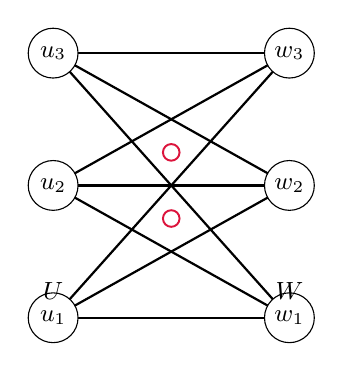
\begin{tikzpicture}[scale=1.2]
    %% K_{3,3} bipartite layout
    \foreach \i/\name in {1/u1,2/u2,3/u3}{
      \coordinate (\name) at (0,{(\i-2)*1.4});
    }
    \foreach \i/\name in {1/w1,2/w2,3/w3}{
      \coordinate (\name) at (2.5,{(\i-2)*1.4});
    }
    %% edges (some cross)
    \foreach \u in {u1,u2,u3}{
      \foreach \w in {w1,w2,w3}{
        \draw[thick] (\u)--(\w);
      }
    }
    %% crossing markers (approximate visual)
    \fill[white] (1.25,0.35) circle (2.5pt);
    \draw[Crimson,line width=0.7pt] (1.25,0.35) circle (2.5pt);
    \fill[white] (1.25,-0.35) circle (2.5pt);
    \draw[Crimson,line width=0.7pt] (1.25,-0.35) circle (2.5pt);
    %% vertex nodes
    \node[vertexW] at (u1) {$u_1$};
    \node[vertexW] at (u2) {$u_2$};
    \node[vertexW] at (u3) {$u_3$};
    \node[vertexW] at (w1) {$w_1$};
    \node[vertexW] at (w2) {$w_2$};
    \node[vertexW] at (w3) {$w_3$};
    %% labels
    \node[above=3pt, font=\small] at (u1) {$U$};
    \node[above=3pt, font=\small] at (w1) {$W$};
  \end{tikzpicture}
  \caption{Left: $K_5$ drawn with five vertices; the circled intersections
           indicate unavoidable edge crossings, confirming non-planarity.
           Right: $K_{3,3}$ in its standard bipartite layout; crossings are
           similarly unavoidable.}
  \label{fig:K5-K33}
\end{figure}

%% ===========================================================
%%  SECTION 3: KURATOWSKI'S THEOREM
%% ===========================================================
\section{Kuratowski's Theorem and Planarity Testing}
\label{sec:kuratowski}

\subsection{Subdivisions and Homeomorphic Graphs}

\begin{definition}[Subdivision]\label{def:subdivision}
  A \textbf{subdivision} of an edge $uv \in E(G)$ is obtained by replacing $uv$
  with a path $u,w,v$, where $w$ is a new vertex of degree $2$.  A
  \textbf{subdivision of a graph} $H$ is a graph obtained from $H$ by
  subdividing any subset of its edges zero or more times.
\end{definition}

\begin{figure}[htbp]
  \centering
  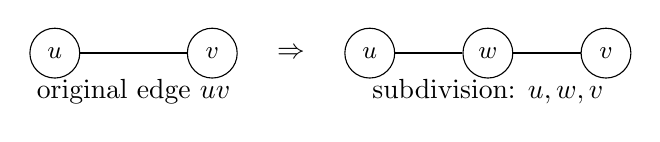
\begin{tikzpicture}
    %% original edge
    \node[vertexW] (u) at (0,0) {$u$};
    \node[vertexW] (v) at (2,0) {$v$};
    \draw[thick] (u)--(v);
    \node[below=6pt] at (1,0) {original edge $uv$};
    %% arrow
    \node at (3,0) {$\Rightarrow$};
    %% subdivided
    \node[vertexW] (u2) at (4,0) {$u$};
    \node[vertexW] (w)  at (5.5,0) {$w$};
    \node[vertexW] (v2) at (7,0) {$v$};
    \draw[thick] (u2)--(w)--(v2);
    \node[below=6pt] at (5.5,0) {subdivision: $u,w,v$};
  \end{tikzpicture}
  \caption{Subdivision of edge $uv$: the new vertex $w$ has degree $2$.}
  \label{fig:subdivision}
\end{figure}

\begin{definition}[Homeomorphic graphs]\label{def:homeomorphic}
  Two graphs $G$ and $H$ are \textbf{homeomorphic} if there exists a graph
  $F$ such that both $G$ and $H$ can be obtained from $F$ by a sequence of
  edge subdivisions.  Equivalently, $G$ and $H$ are homeomorphic if and only
  if they have the same \emph{underlying simple graph} after suppressing all
  degree-$2$ vertices.
\end{definition}

\subsection{Graph Minors}

\begin{definition}[Graph minor]\label{def:minor}
  A graph $H$ is a \textbf{minor} of $G$, written $H \preceq G$, if $H$ can
  be obtained from $G$ by a (possibly empty) sequence of the following
  operations:
  \begin{enumerate}
    \item \textbf{Edge deletion:} remove an edge from the graph.
    \item \textbf{Vertex deletion:} remove a vertex (and all incident edges).
    \item \textbf{Edge contraction:} merge the two endpoints of an edge into a
          single vertex, removing the edge and any resulting multi-edges.
  \end{enumerate}
\end{definition}

\subsection{Kuratowski's and Wagner's Theorems}

\begin{theorem}[Kuratowski, 1930]\label{thm:kuratowski}
  A graph $G$ is planar if and only if it contains no subgraph homeomorphic to
  $K_5$ or $K_{3,3}$.
\end{theorem}

\begin{remark}\label{rem:kuratowski-proof}
  The ``only if'' direction (planar $\Rightarrow$ no forbidden subgraph) follows
  from Corollaries~\ref{cor:K5} and~\ref{thm:K33-nonplanar} together with the
  observation that subdivisions preserve planarity.  The ``if'' direction
  (no forbidden subgraph $\Rightarrow$ planar) is the deep combinatorial content
  of the theorem; see Diestel~\cite{diestel2017} for a complete proof.
\end{remark}

\begin{theorem}[Wagner, 1937]\label{thm:wagner}
  A graph $G$ is planar if and only if it does not contain $K_5$ or $K_{3,3}$
  as a minor.
\end{theorem}

\begin{remark}\label{rem:planarity-algorithms}
  While Theorem~\ref{thm:kuratowski} provides a complete structural
  characterisation of planarity, searching exhaustively for homeomorphic
  subgraphs is computationally expensive.  In practice, \textbf{linear-time
  planarity testing algorithms} are used; the landmark result is due to
  Hopcroft and Tarjan (1974), which decides planarity of an $n$-vertex graph
  in $O(n)$ time.
\end{remark}

\subsection{The Petersen Graph}

\begin{example}[Petersen graph is non-planar]\label{ex:petersen}
  The Petersen graph (Figure~\ref{fig:petersen}) is a well-known $3$-regular
  graph on $10$ vertices and $15$ edges.  It is non-planar: one can exhibit a
  $K_{3,3}$ minor by contracting appropriate edges.  By Theorem~\ref{thm:wagner},
  this confirms non-planarity.
\end{example}

\begin{figure}[htbp]
  \centering
  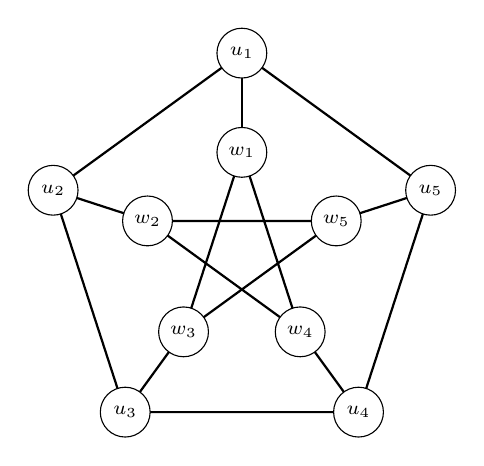
\begin{tikzpicture}[scale=1.4]
    %% Outer pentagon
    \foreach \i/\n in {1/o1,2/o2,3/o3,4/o4,5/o5}{
      \coordinate (\n) at ({90+(\i-1)*72}:1.8cm);
    }
    %% Inner pentagram
    \foreach \i/\n in {1/i1,2/i2,3/i3,4/i4,5/i5}{
      \coordinate (\n) at ({90+(\i-1)*72}:0.9cm);
    }
    %% Outer cycle
    \draw[thick] (o1)--(o2)--(o3)--(o4)--(o5)--(o1);
    %% Spokes
    \foreach \i in {1,2,3,4,5}{
      \draw[thick] (o\i)--(i\i);
    }
    %% Inner pentagram (connect every other)
    \draw[thick] (i1)--(i3)--(i5)--(i2)--(i4)--(i1);
    %% Vertices
    \foreach \n/\lbl in {o1/$u_1$,o2/$u_2$,o3/$u_3$,o4/$u_4$,o5/$u_5$,
                          i1/$w_1$,i2/$w_2$,i3/$w_3$,i4/$w_4$,i5/$w_5$}{
      \node[vertexW, font=\scriptsize] at (\n) {\lbl};
    }
  \end{tikzpicture}
  \caption{The Petersen graph: $10$ vertices, $15$ edges, $3$-regular.  It is
           non-planar; it contains $K_{3,3}$ as a minor (by contracting edges
           $u_1u_2$, $u_3u_4$, and two spokes).}
  \label{fig:petersen}
\end{figure}

%% ===========================================================
%%  SECTION 4: VERTEX COLORING
%% ===========================================================
\section{Graph Coloring — Vertex Coloring}
\label{sec:vertex-coloring}

\begin{definition}[Proper vertex coloring]\label{def:vertex-coloring}
  A \textbf{proper vertex coloring} of a graph $G=(V,E)$ with colors from a
  set $C$ is a function $\phi\colon V \to C$ such that $\phi(u) \neq \phi(v)$
  whenever $uv \in E$.
\end{definition}

\begin{definition}[Chromatic number]\label{def:chromatic}
  The \textbf{chromatic number} of $G$, denoted $\chi(G)$, is the minimum
  cardinality $|C|$ of a color set $C$ admitting a proper vertex coloring of
  $G$.
\end{definition}

\subsection{Standard Examples}

\begin{example}\label{ex:chromatic-examples}
  The following chromatic numbers are standard:
  \begin{enumerate}[label=(\alph*)]
    \item $\chi(K_n) = n$, since every pair of vertices is adjacent.
    \item $\chi(C_n) = 2$ if $n$ is even; $\chi(C_n) = 3$ if $n$ is odd.
    \item $\chi(G) = 2$ for any bipartite graph $G$ (with at least one edge).
    \item $\chi(T) = 2$ for any tree $T$ (with at least one edge), since trees
          are bipartite.
    \item $\chi(G) = 1$ if and only if $G$ has no edges (empty graph).
  \end{enumerate}
\end{example}

\subsection{Bounds on the Chromatic Number}

Let $\omega(G)$ denote the \textbf{clique number} of $G$ (size of the largest
complete subgraph) and $\Delta(G)$ the \textbf{maximum degree}.

\begin{proposition}\label{prop:clique-bound}
  For any graph $G$, $\omega(G) \leq \chi(G)$.
\end{proposition}

\begin{proof}
  Within a clique of size $\omega(G)$, every vertex is adjacent to every other;
  thus all $\omega(G)$ vertices must receive distinct colors.
\end{proof}

\begin{proposition}[Greedy bound]\label{prop:greedy}
  For any graph $G$, $\chi(G) \leq \Delta(G) + 1$.
\end{proposition}

\begin{proof}
  Order the vertices $v_1,\ldots,v_n$ arbitrarily.  Color $v_i$ with the
  smallest positive integer not already used by its earlier neighbors.  When
  coloring $v_i$, at most $\Delta(G)$ earlier neighbors can occupy colors, so
  color $\Delta(G)+1$ is always available.
\end{proof}

\begin{theorem}[Brooks, 1941]\label{thm:brooks}
  Let $G$ be a connected simple graph.  If $G$ is neither a complete graph nor
  an odd cycle, then $\chi(G) \leq \Delta(G)$.
\end{theorem}

\begin{remark}\label{rem:brooks-sketch}
  The proof proceeds by ordering vertices cleverly so that the greedy argument
  requires only $\Delta(G)$ colors.  Specifically, one finds a vertex $v$ such
  that $G - v$ is connected, then applies a greedy coloring starting from $v$
  last.  The key case analysis shows that in the non-exceptional cases a
  color is always saved.  A complete proof appears in Diestel~\cite{diestel2017},
  Chapter~5.
\end{remark}

\begin{figure}[htbp]
  \centering
  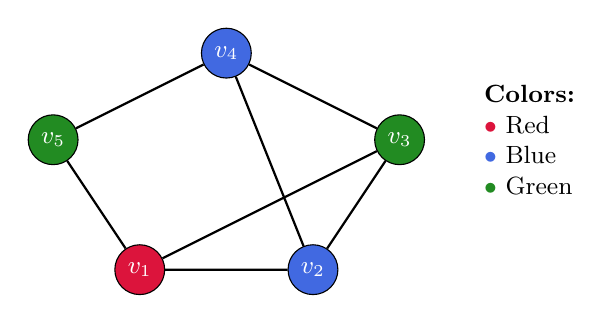
\begin{tikzpicture}[scale=1.1]
    %% A 5-vertex graph with a proper 3-coloring
    \node[redV]    (v1) at (0,0)    {$v_1$};
    \node[blueV]   (v2) at (2,0)    {$v_2$};
    \node[greenV]  (v3) at (3,1.5)  {$v_3$};
    \node[blueV]   (v4) at (1,2.5)  {$v_4$};
    \node[greenV]  (v5) at (-1,1.5) {$v_5$};
    %% edges
    \draw[thick] (v1)--(v2) (v2)--(v3) (v3)--(v4)
                 (v4)--(v5) (v5)--(v1) (v1)--(v3) (v2)--(v4);
    %% color legend
    \node[right=0.4cm, align=left, font=\small] at (3.5,1.5) {%
      \textbf{Colors:}\\
      \textcolor{Crimson}{$\bullet$} Red\\
      \textcolor{RoyalBlue}{$\bullet$} Blue\\
      \textcolor{ForestGreen}{$\bullet$} Green%
    };
  \end{tikzpicture}
  \caption{A proper $3$-coloring of a $5$-vertex graph.  No two adjacent
           vertices share a color.  One can verify $\chi(G)=3$ (the graph
           contains an odd cycle $v_1v_2v_3v_1$... actually triangle
           $v_1,v_2,v_3$ — wait: check edges to confirm $\chi \geq 3$).}
  \label{fig:3-coloring}
\end{figure}

%% ===========================================================
%%  SECTION 5: FOUR COLOR THEOREM
%% ===========================================================
\section{The Four Color Theorem and Planar Graph Coloring}
\label{sec:four-color}

\subsection{Historical Context}

The problem of coloring maps so that adjacent regions receive distinct colors
was posed by Francis Guthrie in $1852$.  The conjecture that four colors always
suffice remained open for over a century, attracting numerous flawed ``proofs''.

\begin{theorem}[Four Color Theorem — Appel \& Haken, 1976]\label{thm:4ct}
  Every simple planar graph is $4$-colorable: for any simple planar graph $G$,
  \[
    \chi(G) \leq 4.
  \]
\end{theorem}

\begin{remark}\label{rem:4ct-proof}
  The proof by Appel and Haken was the first major proof to rely on computer
  assistance, reducing the problem to a finite case check of $1\,936$
  ``unavoidable configurations''.  A simplified (though still
  computer-dependent) proof was given in $1997$ by Robertson, Sanders, Seymour,
  and Thomas.  No purely human-verifiable proof is known.
\end{remark}

\subsection{The Six Color Theorem}

We provide a complete proof of the weaker Six Color Theorem, which uses only
elementary tools developed thus far.

\begin{theorem}[Six Color Theorem]\label{thm:6ct}
  Every simple planar graph $G$ satisfies $\chi(G) \leq 6$.
\end{theorem}

\begin{proof}
  We proceed by induction on $|V(G)| = n$.

  \medskip\noindent
  \textbf{Base case.}  For $n \leq 6$, assign each vertex a distinct color;
  six colors suffice trivially.

  \medskip\noindent
  \textbf{Inductive step.}  Assume every simple planar graph on fewer than $n$
  vertices is $6$-colorable.  By Corollary~\ref{cor:deg5}, $G$ contains a
  vertex $v$ with $\deg(v) \leq 5$.  The induced subgraph $G' = G - v$ is a
  planar graph on $n-1$ vertices.  By the inductive hypothesis, $G'$ admits a
  proper $6$-coloring $\phi$.

  Now we extend $\phi$ to $v$: since $\deg(v) \leq 5$, the vertex $v$ has at
  most $5$ neighbors, which use at most $5$ of the $6$ available colors.
  Therefore at least one color remains available for $v$, and we assign it to
  $v$.  This yields a proper $6$-coloring of $G$.
\end{proof}

\subsection{The Five Color Theorem}

\begin{theorem}[Five Color Theorem — Heawood, 1890]\label{thm:5ct}
  Every simple planar graph $G$ satisfies $\chi(G) \leq 5$.
\end{theorem}

\begin{proof}[Proof sketch]
  Proceed by induction on $|V(G)|$.  As in the proof of
  Theorem~\ref{thm:6ct}, find a vertex $v$ with $\deg(v) \leq 5$ and
  $5$-color $G - v$ by induction.  If $v$ has fewer than $5$ neighbors, at
  least one color is free and we extend immediately.

  The interesting case is $\deg(v) = 5$, with all $5$ neighbors $u_1,\ldots,u_5$
  (in cyclic order around $v$) receiving all $5$ distinct colors $c_1,\ldots,c_5$.
  Consider the induced subgraph on vertices colored $c_1$ or $c_3$.  If $u_1$
  and $u_3$ lie in \emph{different} connected components of this subgraph, we
  can swap colors $c_1 \leftrightarrow c_3$ in $u_1$'s component, freeing color
  $c_1$ at $u_1$ and thus making it available for $v$.  If $u_1$ and $u_3$ lie
  in the \emph{same} component, there is a path $P$ from $u_1$ to $u_3$ using
  only colors $c_1$ and $c_3$.  This path together with the edges $vu_1$,
  $vu_3$ forms a closed curve separating $u_2$ from $u_4$ and $u_5$.
  Consequently, $u_2$ and $u_4$ lie in different components of the
  $(c_2,c_4)$-subgraph, and we may swap colors there to free $c_2$ for $v$.
  In either case, $v$ can be colored.
\end{proof}

\begin{figure}[htbp]
  \centering
  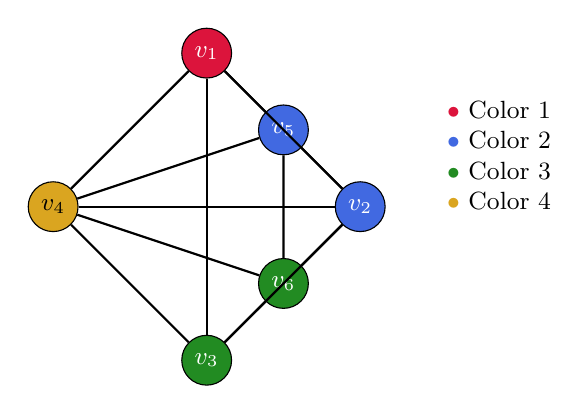
\begin{tikzpicture}[scale=1.3]
    %% A maximal planar graph (octahedron) that requires 4 colors
    %% Vertices
    \node[redV]    (v1) at (0,1.5)   {$v_1$};
    \node[blueV]   (v2) at (1.5,0)   {$v_2$};
    \node[greenV]  (v3) at (0,-1.5)  {$v_3$};
    \node[yellowV] (v4) at (-1.5,0)  {$v_4$};
    \node[blueV]   (v5) at (0.75,0.75) {\small$v_5$};
    \node[greenV]  (v6) at (0.75,-0.75) {\small$v_6$};
    %% outer quad + diagonals
    \draw[thick] (v1)--(v2)--(v3)--(v4)--(v1);
    \draw[thick] (v1)--(v3);
    \draw[thick] (v2)--(v4);
    %% inner connections
    \draw[thick] (v5)--(v1) (v5)--(v2) (v5)--(v4);
    \draw[thick] (v6)--(v2) (v6)--(v3) (v6)--(v4);
    \draw[thick] (v5)--(v6);
    %% legend
    \node[right=0.2cm, align=left, font=\small] at (2.1,0.5) {%
      \textcolor{Crimson}{$\bullet$} Color 1\\
      \textcolor{RoyalBlue}{$\bullet$} Color 2\\
      \textcolor{ForestGreen}{$\bullet$} Color 3\\
      \textcolor{Goldenrod}{$\bullet$} Color 4%
    };
  \end{tikzpicture}
  \caption{A planar graph with a proper $4$-coloring.  All four colors are
           necessary: the subgraph induced by $\{v_1,v_2,v_3,v_4\}$ contains
           $K_4$ (the diagonals $v_1v_3$ and $v_2v_4$ are present), so at
           least $4$ colors are required.}
  \label{fig:4-coloring}
\end{figure}

\begin{remark}\label{rem:3-insufficient}
  The graph in Figure~\ref{fig:4-coloring} requires $4$ colors because it
  contains $K_4$ as a subgraph (vertices $v_1, v_2, v_3, v_4$ are mutually
  adjacent via the edges $v_1v_2, v_2v_3, v_3v_4, v_4v_1, v_1v_3, v_2v_4$).
  By Proposition~\ref{prop:clique-bound}, $\chi(G) \geq \omega(G) = 4$, so
  $3$ colors are provably insufficient.
\end{remark}

%% ===========================================================
%%  SECTION 6: EDGE COLORING
%% ===========================================================
\section{Edge Coloring and Chromatic Index}
\label{sec:edge-coloring}

\begin{definition}[Proper edge coloring]\label{def:edge-coloring}
  A \textbf{proper edge coloring} of a graph $G=(V,E)$ with colors from a set
  $C$ is a function $\psi\colon E \to C$ such that $\psi(e) \neq \psi(f)$
  whenever $e$ and $f$ share a common endpoint.
\end{definition}

\begin{definition}[Chromatic index]\label{def:chromatic-index}
  The \textbf{chromatic index} (or \textbf{edge-chromatic number}) of $G$,
  denoted $\chi'(G)$, is the minimum cardinality of a color set admitting a
  proper edge coloring of $G$.
\end{definition}

\begin{proposition}\label{prop:edge-lower}
  For any graph $G$, $\chi'(G) \geq \Delta(G)$.
\end{proposition}

\begin{proof}
  All edges incident to a vertex of maximum degree $\Delta(G)$ must receive
  distinct colors; hence at least $\Delta(G)$ colors are needed.
\end{proof}

\subsection{Vizing's Theorem}

\begin{theorem}[Vizing, 1964]\label{thm:vizing}
  For any simple graph $G$,
  \[
    \Delta(G) \leq \chi'(G) \leq \Delta(G) + 1.
  \]
\end{theorem}

\begin{remark}\label{rem:vizing-proof}
  The upper bound is the non-trivial content.  The proof proceeds by augmenting
  a partial edge coloring using alternating paths (Kempe chains for edges).
  A complete proof appears in~\cite{diestel2017}.
\end{remark}

\begin{definition}[Class 1 and Class 2 graphs]\label{def:class12}
  A simple graph $G$ is called:
  \begin{itemize}
    \item \textbf{Class~1} if $\chi'(G) = \Delta(G)$;
    \item \textbf{Class~2} if $\chi'(G) = \Delta(G) + 1$.
  \end{itemize}
\end{definition}

\begin{example}[Complete graphs]\label{ex:Kn-edge}
  For the complete graph $K_n$:
  \begin{itemize}
    \item If $n$ is \emph{even}: $\chi'(K_n) = n - 1 = \Delta(K_n)$, so $K_n$
          is \textbf{Class~1}.
    \item If $n$ is \emph{odd} ($n \geq 3$): $\chi'(K_n) = n = \Delta(K_n)+1$,
          so $K_n$ is \textbf{Class~2}.
  \end{itemize}
\end{example}

\begin{example}[Odd cycles]\label{ex:odd-cycle-edge}
  An odd cycle $C_{2k+1}$ ($k \geq 1$) has $\Delta = 2$.  By
  Vizing's Theorem, $2 \leq \chi'(C_{2k+1}) \leq 3$.  Since $C_{2k+1}$ has an
  odd number of edges and each color class is a matching of even cardinality in a
  bipartite graph — but $C_{2k+1}$ is not bipartite — one can show that $2$
  colors do not suffice, so $\chi'(C_{2k+1}) = 3$.  Hence odd cycles are
  \textbf{Class~2}.
\end{example}

\subsection{König's Line Coloring Theorem}

\begin{theorem}[König, 1916]\label{thm:konig}
  For any bipartite graph $G$, $\chi'(G) = \Delta(G)$.  In particular, every
  bipartite graph is Class~1.
\end{theorem}

\begin{proof}[Proof sketch]
  The result follows from König's theorem on perfect matchings in bipartite
  graphs: every regular bipartite graph has a perfect matching.  By iteratively
  decomposing a $\Delta$-regular bipartite supergraph (obtained by adding
  isolated vertices and a dummy edge to regularize) into perfect matchings, one
  obtains a proper edge coloring with $\Delta$ colors.
\end{proof}

\begin{figure}[htbp]
  \centering
  %% K_{3,3} with 3-edge-coloring
  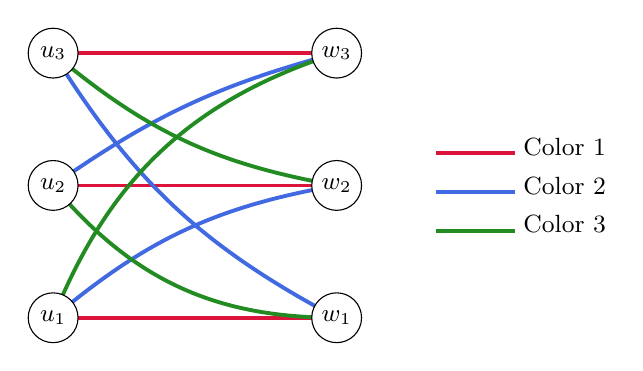
\begin{tikzpicture}[scale=1.2]
    \foreach \i/\n in {1/u1,2/u2,3/u3}{
      \coordinate (\n) at (0,{(\i-2)*1.4});
    }
    \foreach \i/\n in {1/w1,2/w2,3/w3}{
      \coordinate (\n) at (3,{(\i-2)*1.4});
    }
    %% Matching 1 (red): u1-w1, u2-w2, u3-w3
    \draw[edge1] (u1)--(w1);
    \draw[edge1] (u2)--(w2);
    \draw[edge1] (u3)--(w3);
    %% Matching 2 (blue): u1-w2, u2-w3, u3-w1
    \draw[edge2] (u1) to[bend left=15] (w2);
    \draw[edge2] (u2) to[bend left=10] (w3);
    \draw[edge2] (u3) to[bend right=15] (w1);
    %% Matching 3 (green): u1-w3, u2-w1, u3-w2
    \draw[edge3] (u1) to[bend left=25] (w3);
    \draw[edge3] (u2) to[bend right=25] (w1);
    \draw[edge3] (u3) to[bend right=15] (w2);
    %% vertices
    \foreach \n/\lbl in {u1/$u_1$,u2/$u_2$,u3/$u_3$}{
      \node[vertexW,font=\small] at (\n) {\lbl};
    }
    \foreach \n/\lbl in {w1/$w_1$,w2/$w_2$,w3/$w_3$}{
      \node[vertexW,font=\small] at (\n) {\lbl};
    }
    %% legend
    \node[right=0.3cm, align=left, font=\small] at (3.7,0) {%
      \textcolor{Crimson}{\rule{1cm}{1.4pt}} Color 1\\[3pt]
      \textcolor{RoyalBlue}{\rule{1cm}{1.4pt}} Color 2\\[3pt]
      \textcolor{ForestGreen}{\rule{1cm}{1.4pt}} Color 3%
    };
  \end{tikzpicture}
  \hspace{1.5cm}
  %% Odd cycle C5 with 3-edge-coloring
  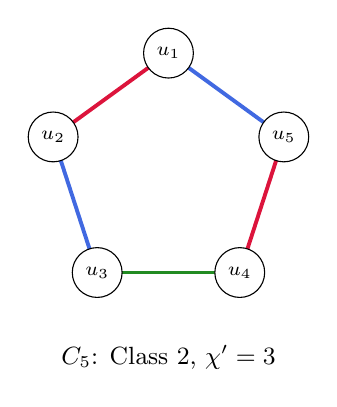
\begin{tikzpicture}[scale=1.1]
    \foreach \i/\n in {1/p1,2/p2,3/p3,4/p4,5/p5}{
      \coordinate (\n) at ({90+(\i-1)*72}:1.4cm);
    }
    \draw[edge1] (p1)--(p2);
    \draw[edge2] (p2)--(p3);
    \draw[edge3] (p3)--(p4);
    \draw[edge1] (p4)--(p5);
    \draw[edge2] (p5)--(p1);
    \foreach \n/\lbl in {p1/$u_1$,p2/$u_2$,p3/$u_3$,p4/$u_4$,p5/$u_5$}{
      \node[vertexW,font=\scriptsize] at (\n) {\lbl};
    }
    \node[below=0.5cm, font=\small] at (0,-1.4) {$C_5$: Class 2, $\chi'=3$};
  \end{tikzpicture}
  \caption{Left: Proper $3$-edge-coloring of $K_{3,3}$ ($\Delta=3$, Class~1
           by König's theorem).  Each color class is a perfect matching.
           Right: Proper $3$-edge-coloring of $C_5$ ($\Delta=2$,
           $\chi'=3$, Class~2).}
  \label{fig:edge-coloring}
\end{figure}

\end{document}